\documentclass{article}

\usepackage{amssymb}
\usepackage{polski}
\usepackage[polish]{babel}
\usepackage[utf8]{inputenc}
\usepackage{amsmath}
\usepackage{hyperref}
\usepackage{graphicx}

\title{Aplikacja do śledzenia celów i fuzji danych  \\ {\large Dokumentacja końcowa}}
\author{Przemysław Saramonowicz, Marcin Buczko, Jacek Palczewski \\ Wydział Elektroniki i Technik Informacyjnych \\ Politechnika Warszawska}
\date{26 stycznia 2015 r.}
%wypełnienie strony
%\setlength{\textheight}{24cm}
%\setlength{\textwidth}{15.92cm}
%\setlength{\footskip}{10mm}
%\setlength{\oddsidemargin}{0mm}
%\setlength{\evensidemargin}{0mm}
%\setlength{\topmargin}{0mm}
%\setlength{\headsep}{5mm}

%kropki po \section
\usepackage{titlesec}
\titlelabel{\thetitle.\quad}

\begin{document}
	\maketitle
	
	\section{Realizacja zagadnień}
		Podsumowanie zostanie oparte o punkty z dokumentacji wstępnej, które zostaną skomentowane na podstawie bieżących etapów prac.	
		\begin{itemize}
		\item \textbf{Symulacja ruchu obiektu} - obiekt będzie poruszał się w przestrzeni dwuwumiarowej po zdefiniowanych wcześniej trajektoriach ruchu oraz przekazywał dane o swoim położeniu sensorom.
		\begin{itemize}
			\item Ten moduł programu udało się zrealizować w zadowalającym stopniu: trajektoria obiektu jest generowana w oparciu o skrypty w języku Python(katalog \texttt{maps/}).
		\end{itemize}

		\item \textbf{Sensor ruchu} - odbiera dane o położeniu obiektu i przekazuje je razem z własnym szumem pomiarowym na wejście filtru Kalmana.
			\begin{itemize}
				\item Miejsce na komentarze... 
			\end{itemize}

		\item \textbf{Filtr Kalmana} - Odbiera dane z sensorów i wyznacza stan wewnętrzny modelowanego obiektu
			\begin{itemize}
				\item Miejsce na komentarze... 
			\end{itemize}
		
		\item \textbf{Moduł określający błąd pomiaru} - Odbiera dane od obiektu, sensorów oraz filtru Kalmana i określa jak dokładnie filtr Kalmana przewiduje tor w kolejnych iteracjach oraz określa poprawę w stosunku do odczytów sensorów.
			\begin{itemize}
				\item Moduł został połączony z poniższym, por. punkt niżej i dalsze rozdziały.
			\end{itemize}
				
		\item \textbf{Interpretacja graficzna działania programu} - Rysuje obiekt w kolejnych iteracjach na jego pozycji oraz jego kopię w miejscu określonym przez układ sensorów z filtrem Kalmana a także trajektorię obu instancji obiektu.
			\begin{itemize}
				\item Mimo pierwotnych planów o zrealizowaniu tego modułu w języku C++, ze względu na problemy z implementacją wyświetlania wyników symulacji w czasie rzeczywistym Zespół podjął decyzję o zmianie podejścia: program składający się z pozostałych modułów jest zrealizowany jako aplikacja w C++, a bieżący moduł został napisany jako uniwersalny skrypt do środowiska Octave(kompatybilnego z Matlabem). Dokładne działanie całego projektu zostanie opisane później.
			\end{itemize}
			
		\item Zależność pomiędzy torem ruchu i prędkością a dokładnością pomiaru; wpływ ilości sensorów na dokładność odczytu. 
			\begin{itemize}
				\item Możliwość uruchomienia z innym torem obiektu(jak również zmiany współczynników - pliki .ini) w opinii Zespołu realizuje olbrzymią część tego założenia.
				\item Miejsce na komentarze... 
			\end{itemize}
		\item Przenośność pomiędzy Windowsem a Linuxem.
			\begin{itemize}
				\item Był to podpunkt intrygujący ze względu na wiele niespodzianek( głównie ze względu na ciekawe różnice pomiędzy kompilatorami( Visual Studio jest o wiele bardziej liberalny i różni się subtelnościami w implementacji niektórych rzeczy nawet w bibliotece standardowej: dla przykładu konstruktor \texttt{std::exception} przyjmujący ciągi znaków pod MSVC, który nie jest dozwolony w GCC - tam identyczną funkcję pełni \texttt{std::runtime\_error})), aczkolwiek dzięki wykorzystaniu Jenkinsa udało się utrzymać ten podpunkt. 
			\end{itemize}
				
		\end{itemize}		
	
	\section{Opis stanu prac nad projektem}
	
	\subsection{Rozwiązania zastosowane w projekcie - synchronizacja, etc.}
		\subsubsection{Klasa Worker}
		 Problem synchronizacji dotyczył praktycznie każdego modułu w aplikacji opartej na wątkach, dlatego został rozwiązany globalnie, poprzez klasę \texttt{Worker<T>}, która korzysta z dobrodziejstw programowania generycznego, czyli trejtów, uproszczając całą obsługę synchronizacji do przeciążenia funkcji \texttt{ThreadProc} w module dziedziczącym po w.w. klasie, a obsługa zmiennej warunkowej, kolejki i synchronizacji jest w gestii kompilatora dla wielu różnych, różniących się szczegółami klas.
		 
	\newpage 
	\subsection{Jak program działa - opis}
	\begin{enumerate}
		\item Aplikacja
		\begin{verse} 
			Aplikację można uruchomić z konsoli, bądź poprzez skrypty \texttt{runme}, dzięki czemu automatycznie zostanie uruchomiony punkt 6 po zakończonej symulacji.
		\end{verse}
		\item Generator
		 \begin{verse}
		 \texttt{Worker<OutputWorker>} uruchamia przeciążoną funkcję ThreadProc, która natomiast wywołuje skrypt który jest załadowany z pliku - za pomocą wyrażeń regularnych jest przeprowadzone wstępne sprawdzenie czy skrypt jest prawidłowy(tj. czy istnieje funkcja która ma taką samą nazwę co plik w celu weryfikacji) jest cyklicznie uruchamiana i wszystkie obliczenia są przeprowadzane w środowisku Python(dzięki czemu między wywołaniami funkcji w Pythonie możemy przechowywać dane w zmiennych globalnych - por. pliki w katalogu \texttt{maps/}, a biblioteka \texttt{Booost::python} pozwala na załadowanie tych wyników i dalsze przetwarzanie.
		 \end{verse}
		\item Sensor
		\begin{verse}
		SENSOR OPIS TUTEJ
		\end{verse}
		\item Kalman
		\begin{verse}
		KALMAN OPIS TUTEJ
		\end{verse}
		\item Writer
		\begin{verse}
		Zespół podjął decyzję o przechowywaniu wartości w plikach CSV\footnote{ang. \textit{Comma separated values} - mimo nazwy separatorem zostały średniki, wybrane w celu zachowania zgodności z aplikacją Excel, która była wstępnie wykorzystywania do analizy wyników.} ze względu na prostotę formatu. 
		\end{verse}
		\item Skrypty Matlab 
		\begin{verse}
		Z powstałego pliku .csv skrypt \texttt{script.m} wczytuje współrzędne
		punktów wygenerowanych w trakcie symulacji przez program,
		oblicza odchylenie standardowe różnic wartości współrzędnych
		x, y dla czujnika i filtra kalmana oraz rysuje 3 wykresy : 
		\begin{enumerate}
			\item wartości zmiennych \texttt{X} dla generatora, czujnika i filtru Kalmana;
			\item wartości zmiennych \texttt{Y} dla generatora, czujnika i filtru Kalmana;
			\item torów ruchu na podstawie odczytu generatora, czujnika i filtru Kalmana.
		\end{enumerate}
		W celu uruchomienia programu z tą funkcją należy wywołać skrypt \texttt{runme.bat} (lub \texttt{runme.sh} dla systemów linuxowych) w argumentach podając mu ścieżkę do skryptu pythona dla interesującej nas trajektorii oraz wywołanie funkcji w języku Matlab np. \texttt{runme.bat ../maps/standard acc.py script(1000)}. Argumentem w przypadku skryptu \texttt{script.m} jest ilość punktów rysowanych na wykresie.
		\end{verse}
	\end{enumerate}
	
	\section{Napotkane problemy, popełnione błędy, wnioski}
	
	\subsection{Problemy i błędy napotkane podczas pisania}
	\subsubsection{Rozbieżności pomiędzy MSVC i GCC}
	Pisanie aplikacji dostępnym na wiele platform jest procesem dość wymagającym głównie ze względu na fakt, że MSVC jest, jak już zostało wspomniane wcześniej, kompilatorem dość liberalnym - pozwala na dużo rozwiązań które nie są możliwe jeżeli przychodzi co do kompilacji pod GCC. Dlatego cennym rozwiązaniem było skorzystanie Github Student Pack\footnote{\url{https://education.github.com/pack}}, dzięki któremu Zespół uzyskał dostęp do darmowej maszyny wirtualnej która pozwoliła na zainstalowanie instancji Jenkinsa działającej 24/7 - CI pozwalało śledzić czy każdy nowy commit(zwykle projektowany pod Windowsem) kompiluje się pod Linuxem - dlatego dość szybko można było w stanie wykryć poniższy błąd.
	\subsubsection{GCC i argument określany przez typedef}
	Tutaj Zespół spotkał się z dość dziwnym błędem - GCC nie pozwalało na określanie argumentu funkcji jako typ \texttt{void} w przeciwieństwie do MSVC  który zezwala na taką operację, dlatego trejt \texttt{CommonUtil::Traits::InputWorker} definiuje typ argumentu funkcji \texttt{ThreadProc} jako int.

	\subsubsection{Rozbieżności pomiędzy szkieletem a aplikacją końcową.}
	Mimo początkowych planów skorzystania z bibliotek SDL i wxWidgets w finalnej wersji nie zostały użyte, głównie ze względu na to, że wyświetlanie komórek w czasie rzeczywistym jest procesem dość złożonym tak samo jak próba wpływu na zmiany na parametry symulacji. 
	
	\subsubsection{Automatyzacja liczenia pokrycia kodu.}
	Mimo próby podejścia do automatyzacji(por. przełącznik coverage w pliku \texttt{SConscript}) liczenia pokrycia kodu nie udało się osiągnąć zadowalających rezultatów.
	
	\subsection{Wnioski, rozwiązania}
 	
 	\subsubsection{Automatyzacja testowania}
 	Z drugiej strony automatyzacja testów była dość dobra - każda udana kompilacja kończyła się uruchomieniem skryptu \texttt{test\_runner.sh} na jenkisie, co kończyło się generowaniem plików .xml które były potem interpretowane przez wtyczkę do postaci wykresu:
 	
 	
 	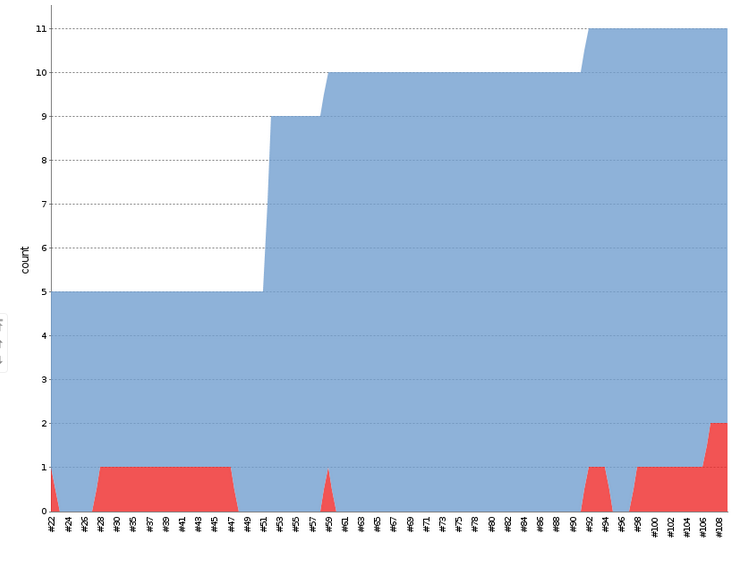
\includegraphics[scale=0.6]{testy} 
 	
 	(Gwoli ścisłości: testy zaznaczone na czerwono odnoszą się do skryptów wykonywanych przy wykorzystaniu ścieżek relatywnych, a plugin w jenkinsie odpowiedzialny za ich wykonanie \textit{ucieka} ze względów bezpieczeństwa do folderu \texttt{/tmp}, przez co takiego testy są skazane na niepowodzenie. )
 	
 	
 	
 	\begin{table}[]
 \centering
\caption{Końcowe statystyki}
\label{my-label}
\begin{tabular}{|l|l|}
\hline
Liczba linijek kodu & 1 \\ \hline
Liczba commitów     & 2 \\ \hline
Liczba testów       & 3 \\ \hline
\end{tabular}
\end{table}
%\begin{thebibliography}{19}
 
%\bibitem{regulamin}
%  Centralne Laboratorium Fizyki Wydziału Fizyki Politechniki Warszawskiej, \\
%  \emph{Regulamin CLF}.
%  Dostęp: 21 marca, 2015 r,   
%  \url{http://clf.if.pw.edu.pl/?q=pl/regulamin-clf}
  
%\end{thebibliography}


\end{document}